\documentclass[a4paper,14pt]{extarticle}


\usepackage[utf8]{inputenc}
\usepackage[T2A]{fontenc}
\usepackage[english,russian]{babel}
\usepackage{ragged2e}
\usepackage[utf8]{inputenc}
\usepackage{hyperref}
\usepackage{minted}
\setmintedinline{frame=lines, framesep=2mm, baselinestretch=1.5, bgcolor=LightGray, breaklines,fontsize=\scriptsize}
\setminted{frame=lines, framesep=2mm, baselinestretch=1.5, bgcolor=LightGray, breaklines,fontsize=\scriptsize}
\usepackage{xcolor}
\definecolor{LightGray}{gray}{0.9}
\usepackage{graphicx}
\usepackage[export]{adjustbox}
\usepackage[left=1cm,right=1cm, top=1cm,bottom=1cm,bindingoffset=0cm]{geometry}
\usepackage{fontspec}
\usepackage{ upgreek }
\usepackage[shortlabels]{enumitem}
\usepackage{adjustbox}
\usepackage{multirow}
\usepackage{amsmath}
\usepackage{amssymb}
\usepackage{pifont}
\usepackage{pgfplots}
\usepackage{longtable}
\usepackage{array}
\graphicspath{ {./images/} }
\makeatletter
\AddEnumerateCounter{\asbuk}{\russian@alph}{щ}
\makeatother
\setmonofont{Consolas}
\setmainfont{Times New Roman}

\newcommand\textbox[1]{
	\parbox{.45\textwidth}{#1}
} 

\newcommand{\specialcell}[2][c]{%
	\begin{tabular}[#1]{@{}c@{}}#2\end{tabular}}

\begin{document}
\pagenumbering{gobble}
\begin{center}
    \small{
        \textbf{МИНИCТЕРCТВО НАУКИ И ВЫCШЕГО ОБРАЗОВАНИЯ РОCCИЙCКОЙ ФЕДЕРАЦИИ}\\
        ФЕДЕРАЛЬНОЕ ГОCУДАРCТВЕННОЕ БЮДЖЕТНОЕ ОБРАЗОВАТЕЛЬНОЕ УЧРЕЖДЕНИЕ\\ВЫCШЕГО ОБРАЗОВАНИЯ \\
        \textbf{«БЕЛГОРОДCКИЙ ГОCУДАРCТВЕННЫЙ ТЕХНОЛОГИЧЕCКИЙ\\УНИВЕРCИТЕТ им. В. Г. ШУХОВА»\\ (БГТУ им. В.Г. Шухова)} \\
        \bigbreak
        
\includegraphics[width=70mm]{log}\\
        ИНСТИТУТ ИНФОРМАЦИОННЫХ ТЕХНОЛОГИЙ И УПРАВЛЯЮЩИХ СИСТЕМ\\}
\end{center}

\vfill
\begin{center}
    \large{
        \textbf{
            Лабораторная работа №4}}\\
    \normalsize{
        по дисциплине: Основы ИИ \\
        тема: «Введение в искусственные нейронные сети»}
\end{center}
\vfill
\hfill\textbox{
    Выполнил: ст. группы ПВ-223\\Пахомов Владислав Андреевич
    \bigbreak
    Проверили: \\пр. Твердохлеб Виталий Викторович
}
\vfill\begin{center}
    Белгород 2025 г.
\end{center}
\newpage
\underline{\textbf{Цель работы: }}разработка и исследование алгоритмов обучения искусственных нейронных сетей.
\begin{center}
\textbf{Ход выполнения работы}
\end{center}

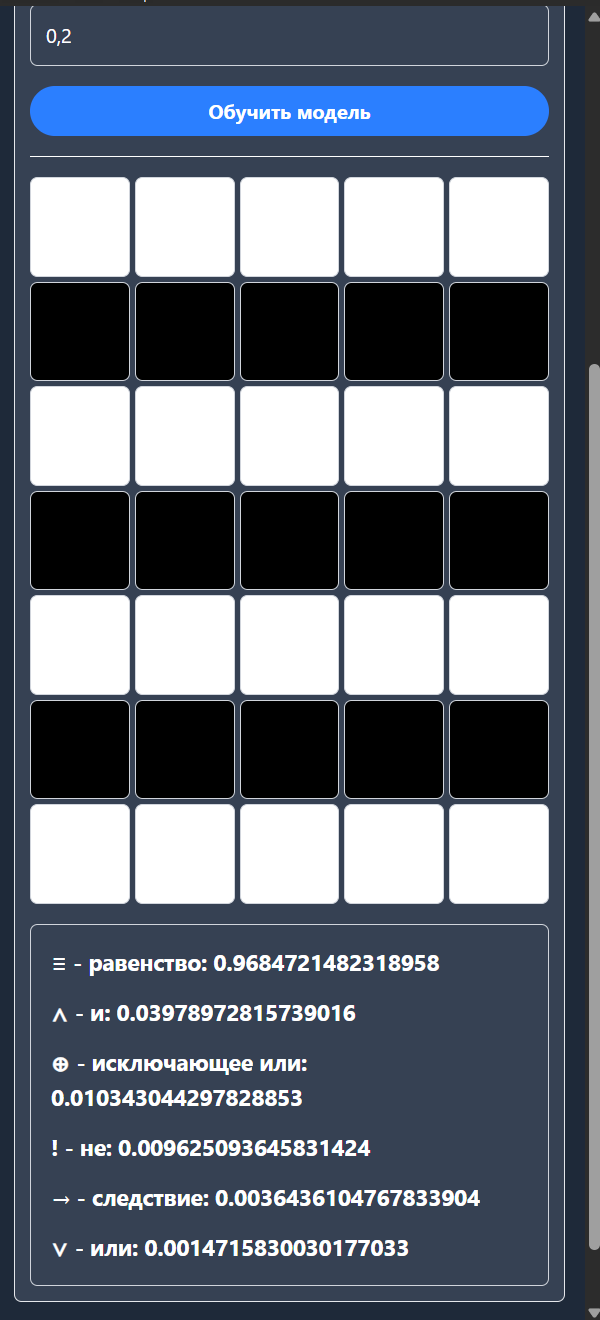
\includegraphics[width=90mm]{demo}\\

\textbf{Вывод:} в ходе лабораторной работы разработали и исследовали алгоритмы обучения искусственных нейронных сетей.

\href{https://github.com/IAmProgrammist/ai_basics/tree/lab4}{Ссылка на репозиторий}\\

\begin{minted}{Rust}
use rand::Rng;
use std::f64::consts::E;

pub const INPUT_NEURONS_WIDTH: usize = 5;
pub const INPUT_NEURONS_HEIGHT: usize = 7;
pub const INPUT_NEURONS: usize = INPUT_NEURONS_WIDTH * INPUT_NEURONS_HEIGHT;
pub const HIDDEN_NEURONS: usize = 5;
pub const OUTPUT_NEURONS: usize = 6;

#[derive(Clone, Copy)]
pub struct NeuralNetwork {
    // Weight Structures (with biases as last elements)
    wih: [[f64; HIDDEN_NEURONS]; INPUT_NEURONS + 1],
    who: [[f64; OUTPUT_NEURONS]; HIDDEN_NEURONS + 1],
    
    // Activations
    inputs: [f64; INPUT_NEURONS],
    hidden: [f64; HIDDEN_NEURONS],
    target: [f64; OUTPUT_NEURONS],
    pub actual: [f64; OUTPUT_NEURONS],
    
    // Unit Errors
    erro: [f64; OUTPUT_NEURONS],
    errh: [f64; HIDDEN_NEURONS],
}

#[derive(Clone, Copy)]
pub struct BackpropElement {
    pub data_in: [f64; INPUT_NEURONS],
    pub out: [f64; OUTPUT_NEURONS],
}

impl NeuralNetwork {
    pub fn new() -> Self {
        let mut res = Self {
            wih: [[0.0; HIDDEN_NEURONS]; INPUT_NEURONS + 1],
            who: [[0.0; OUTPUT_NEURONS]; HIDDEN_NEURONS + 1],
            inputs: [0.0; INPUT_NEURONS],
            hidden: [0.0; HIDDEN_NEURONS],
            target: [0.0; OUTPUT_NEURONS],
            actual: [0.0; OUTPUT_NEURONS],
            erro: [0.0; OUTPUT_NEURONS],
            errh: [0.0; HIDDEN_NEURONS],
        };
        res.assign_random_weights();
        res
    }

    pub fn assign_random_weights(&mut self) {
        let mut rng = rand::thread_rng();
        
        for inp in 0..INPUT_NEURONS + 1 {
            for hid in 0..HIDDEN_NEURONS {
                self.wih[inp][hid] = rng.gen_range(-0.5..0.5);
            }
        }

        for hid in 0..HIDDEN_NEURONS + 1 {
            for out in 0..OUTPUT_NEURONS {
                self.who[hid][out] = rng.gen_range(-0.5..0.5);
            }
        }
    }

    pub fn sigmoid(val: f64) -> f64 {
        1.0 / (1.0 + E.powf(-val))
    }

    pub fn sigmoid_derivative(val: f64) -> f64 {
        val * (1.0 - val)
    }

    pub fn feed_forward(&mut self) {
        // Calculate input to hidden layer
        for hid in 0..HIDDEN_NEURONS {
            let mut sum = 0.0;
            for inp in 0..INPUT_NEURONS {
                sum += self.inputs[inp] * self.wih[inp][hid];
            }

            // Add in Bias
            sum += self.wih[INPUT_NEURONS][hid];

            self.hidden[hid] = Self::sigmoid(sum);
        }

        // Calculate the hidden to output layer
        for out in 0..OUTPUT_NEURONS {
            let mut sum = 0.0;
            for hid in 0..HIDDEN_NEURONS {
                sum += self.hidden[hid] * self.who[hid][out];
            }

            // Add in Bias
            sum += self.who[HIDDEN_NEURONS][out];

            self.actual[out] = Self::sigmoid(sum);
        }
    }

    pub fn back_propagate(&mut self, learn_rate: f64) {
        // Calculate the output layer error
        for out in 0..OUTPUT_NEURONS {
            self.erro[out] = (self.target[out] - self.actual[out]) * 
                             Self::sigmoid_derivative(self.actual[out]);
        }

        // Calculate the hidden layer error
        for hid in 0..HIDDEN_NEURONS {
            self.errh[hid] = 0.0;
            for out in 0..OUTPUT_NEURONS {
                self.errh[hid] += self.erro[out] * self.who[hid][out];
            }

            self.errh[hid] *= Self::sigmoid_derivative(self.hidden[hid]);
        }

        // Update the weights for the output layer
        for out in 0..OUTPUT_NEURONS {
            for hid in 0..HIDDEN_NEURONS {
                self.who[hid][out] += learn_rate * self.erro[out] * self.hidden[hid];
            }

            // Update the Bias
            self.who[HIDDEN_NEURONS][out] += learn_rate * self.erro[out];
        }

        // Update the weights for the hidden layer
        for hid in 0..HIDDEN_NEURONS {
            for inp in 0..INPUT_NEURONS {
                self.wih[inp][hid] += learn_rate * self.errh[hid] * self.inputs[inp];
            }

            // Update the Bias
            self.wih[INPUT_NEURONS][hid] += learn_rate * self.errh[hid];
        }
    }

    pub fn set_inputs(&mut self, sample: &BackpropElement) {
        self.inputs.copy_from_slice(&sample.data_in);
        self.target.copy_from_slice(&sample.out);
    }
}
\end{minted}

\end{document}